\chapter{\uppercase{Ranking Biologically-Interesting SNPs in Incipient Species of Malaria Vectors using Random Forests}}

\section{Abstract}
  \paragraph*{Background:}
  Half of the world's population is at risk for malaria infection through vectors such as the mosquitoes \emph{Anopheles gambiae} and \emph{Anopheles coluzzii}.  Having recently diverged, the two species differ in feeding and mating habits as well as insecticide resistance but cannot be differentiated visually. Identifying genetic differences between the two species is key to understanding the biological differences and designing effective population-control efforts.
  
  \paragraph*{Results:}
  Random Forests have been used in bioinformatics literature to identify subsets of genetic markers that describe phenotypic differences in studies as diverse as cancer and diabetes. 
  We use numerical experiments to illustrate the susceptibility of Random Forests to multiple sources of bias if not used with care, which affect variable importance score accuracy.
  We describe solutions to correct for bias and demonstrate that Random Forests can identify biologically-meaningful biallelic SNPs in insect vectors.
  
  \paragraph*{Conclusion:}
  We demonstrated the utility of Random Forests for analyzing biallelic SNPs in the context of population genetics while also describing multiple sources of bias and their solutions.  We implemented our workflow using Python and scikit-learn and released it under an open-source license for others to use.

\section{Introduction}
The accumulation of genetic differences within separate populations may result in new species. Genetic differences between long-separated species often have macroscopic genomic differences such as re-ordered genes that are relatively easy to detect. During the early stages of speciation, however, genetic differences are often subtle, occurring in the form of differences in allele frequencies or combinations thereof. For example, the apple maggot \emph{Rhagoletis pomonella} separated from \emph{Rhagoletis zepheria} no more than two centuries ago, but allele frequencies likely changed rapidly \cite{Egan2015}.  Another classic example of recent speciation are the malaria vectors \emph{An. gambiae} and \emph{An. coluzzii} that were difficult to distingish genetically even after whole genome sequencing \cite{Lawniczak2010}. Tools and methods for identifying identifying genetic differences are valuable to efforts aiming to molecularly characterize such closely related species and ultimately understand underlying causes of speciation in these model systems.

Genetic differentiation of insects, however, faces several challenges. Although the genome sizes can be relatively small compared to human, collecting and sequencing enough samples is costly for these communities.  Further, many of these species have very little linkage disequilibrium (LD), for which single nucletide polymorphisms (SNPs) tend to be the primary feature (as opposed to larger haplotype blocks in species like human). Combined, currently available data sets tend to be ``wide'' with many features and few samples \cite{Lawniczak2010, Egan2015, Fontaine2015}.

Given the lack of LD, the typical method as applied to insect population genomics involve calculating multiple univariate statistics such as $F_{ST}$, nucleotide diversity ($\pi$), and Tajima's $D$ \cite{Fontaine2015}. Relatively diverged regions are isolated by atypical values, usually visualized across the genome \cite{Egan2015, Fontaine2015}. Due to the relatively small amount of information per SNP, a common strategy is to look at genome intervals (windows) in an attempt to amplify signal. Window-based analysis is able to find interactions between nearby SNPs but not larger interacting regions, especially in the absence of a previously competed reference genome \cite{Egan2015}.

Random Forests (RFs) offer an attractive alternative to more traditional techniques \cite{Breiman1999}. RFs are a versatile machine learning method that can be used for classification (supervised learning), variable selection, regression, and clustering (unsupervised learning).  RFs are able to utilize heterogenous features types such as real numbers or integers, categories, and ordinals. RFs also tend to perform well on data sets with numerous unlinked features such as genome-based SNPs with little LD \cite{Meng2009}.

RFs have started to see adoption across a range of problems in computational biology.  D\'{\i}az-Uriarte, et al. applied RFs to gene selection and classification from microarray data, finding that RFs perform in the case of a large number of noisy features \cite{Diaz-Uriarte2006}. Jiang, et al. successfully applied RFs to the classification of microRNA precursors \cite{Jiang2007}. Chen, et al. used RFs to predict protein-protein interactions \cite{Chen2005}. Kandaaswamy, et al. used RFs to identify anti-freeze proteins from sequence-derived features. RF clustering has been used by Shi, et al. to classify tumors from microarray data \cite{Shi2005}. Lin, et al. and Wu, et al. used RFs to identify DNA-binding proteins \cite{Lin2011}. Jiang, et al. applied RFs to predict SNP interactions associated with Age-related Macular Degeneration in a genome-wide associated study \cite{Jiang2009}. Lunetta, et al. also applied RFs to predicting SNP interactions in a large-scale association study \cite{Lunetta2004}.  Liu, et al. applied RFs to identifying protein-RNA binding sites \cite{Liu2010}. Moore, et al. reviewed computational challenges in genome-wide association studies, arguing for Random Forests as one solution \cite{Moore2010}.

Researchers have begun to identify challenges associated with using RFs for bioinformatics problems and extensions to RF methods. Strobl, et al. identified issues with bias in RF variable importance scores associated with categorical variables and bootstrap resampling of samples during training and proposed a new method called ``cforest'' \cite{Strobl2007}. Nicodemus, et al. analyzed bias present in RF permutation-based variable importance measures \cite{Nicodemus2010}. To overcome identified issues, Strobl, et al. proposed the Conditional Random Forest method \cite{Strobl2008}. Altmann, et al. proposed using permutation importance as variable importance measure that avoids bias present in the more traditional Gini importance measure \cite{Altmann2010}. Calle, et al. compared two common variable importance measures, mean decrease accuracy and mean decrease Gini, finding that mean decrease Gini is more stable in the face of small perturbations \cite{Calle2011}. Amaratunga, et al. proposed using weights so that features are not sampled uniformally in splits, calling the method Enriched Random Forests \cite{Amaratunga2008}.

We consider the problem of apply RFs to challenging whole-genome studies of early speciation of insects. We use simulated data sets to demonstrate that RFs are susceptible to multiple sources of bias, in line with previous work by Strobl, et al \cite{Strobl2007, Strobl2008, Nicodemus2010} and Altmann, et al. \cite{Altmann2010}. Unlike the previous work, we describe a solutions that can be used with common ``out-of-the-box'' implementations of decision trees. We apply our solutions to ranking SNPs, which we validate by identifying SNPs associated with incipient speciation of insect vectors.  Our workflow is implemented in and available through an open-source software package written in Python using the scikit-learn, Numpy, and matplotlib libraries \cite{scikit-learn, Stefan2011,Hunter2007}.


\section{Methods}
\subsection{Simulated Data Sets}
\subsubsection{Encoding Schemes}
We randomly generated 100 datasets with 1000 samples and uninformative 31 categorical variables with 2-32 categories each.  The values of the categorical variables were sampled from an uniform distribution so that each category had an equal chance of being chosen and no correlation with the output labels. Random Forests with 100 trees were trained on each dataset and used to compute variable importance scores.

Under the integer encoding scheme, each of the 31 categorical variables was encoded as a column in the feature matrix with the categories represented as integers starting from 0.  In one-hot encoding, each category variable of $N$ categories is encoded as $N$ binary columns with values of 0 or 1.  The columns are mutually exclusive such that only one of the columns can be ``hot,'' or have value of 1 for each sample.  The resulting feature matrix had 527 columns.  When computing the variable importance score for each one-hot encoded categorical variable, we averaged the variable importance scores from the columns associated with that variable.

\subsubsection{Unknown Genotypes}
Each SNP was encoded as two features, giving the number of As and Ts respectively.  For example, A/A becomes (2, 0), A/T becomes (1, 1), and T/T becomes (0, 2).  The SNPs are organized into four groups of three.  The first three SNPs are chosen from a uniform distribution and uncorrelated with the output labels.  The remaining three groups of SNPs have 100\%, 75\%, and 50\% probabilities, respectively, of being correlated with the output label. To simulate the effect of missing data, we zeroed out the features of the first, second, and third SNP in each group for 0, 10, and 20 randomly-chosen individuals.  We generated 100 datasets with 100 samples each and trained a RF with 100 trees on each dataset.  

\subsubsection{Number of Variables}
We randomly generated data sets of 10 samples with 5, 10, and 25 uncorrelated binary variables.  The output labels were sampled uniformally from $\{0, 1\}$.  Variable importance scores were computed from Random Forests with 100 trees.  We ran 100 simulations.

\subsubsection{Correlated Variables}
We used simulations to evaluate the effect of variable correlation on variable importance scores. We randomly generated data sets of 10 samples with 25 binary variables.  The data sets had 1, 10, and 25 features with values correlated with the output label and each other. The output labels were sampled uniformally from $\{0, 1\}$. Variable importance scores were computed from one Random Forest with 100 trees per simulation.  We ran 100 simulations.

\subsubsection{Confounding Variables}
We randomly generated data sets of ten samples with none binary variables. The data sets had two classes with five samples assigned to each.  Seven of the variables were uncorrelated -- values were chosen uniformally from $\{0, 1\}$. One of the variables was correlated with the output label.  And lastly, one of the variables was correlated with the output label for all but one sample, which had a value equal to the output label for the other class.  Distributions of mean decrease in impurities were calculated using 10,000 decision trees.

\subsection{Workflow for Ranking SNPs with Random Forests}
Our workflow for ranking biallelic SNPs has the following stages: (optional) impute missing genotypes, encode tbe feature matrix, (optional) apply dictionary compression to the feature matrix, train Random Forests, rank the SNPs, and analyze the stability of the rankings.  Our workflow is implemented in the Asaph software using Python and the sci-kit learn library.  Asaph is available under the open-source Apache License v2.

As input, Asaph expects a VCF file containing $M$ phased biallelic SNP variants for $N$ individuals and a file mapping the individuals' IDs to populations (groups or classes). 

\subsubsection{Filtering Uninformative SNPs}
As a preprocessing step, we remove SNPs that are otherwise uninformative.  The class of uninformative SNPs includes those with a single genotype or where an entire group of samples have unknown genotypes.

\subsubsection{Imputing Unknown Genotypes}
To prevent bias, we (optionally) impute unknown genotypes (e.g., X/X, A/X) from known genotypes (e.g., A/A).  Samples are first sorted into their respective groups or classes. For each class, we count the number of occurrences of each known genotype and compute their frequencies by frequencies by dividing by the number of samples with known genotypes.  The known genotype with the highest frequency is used is substituted for the unknown genotypes if its frequency is higher than a user-provided threshold.  The threshold is employed to prevent imputation in situations with low levels of certainty.

Consider the example data for two groups of samples with a single SNP in Table~\ref{tab:unknown-genotypes-example}.  Let's look at imputing the unknown genotypes with a threshold of 100\%. For group 1, the genotype A/T has the highest frequency at 100\%, which satisfies the threshold.  The unknown genotype X/X for sample 4 would be replaced with A/T.  For group 2, the most-frequent genotype of the two is A/A, but it only has a frequency of 66.7\%, which does not satisfy the threshold.  As a result, sample 8's unknown genotype would not be replaced.

\subsubsection{Feature Matrix Encoding}
After unknown genotypes are imputed, the SNP data is transformed into a feature matrix suitable for Random Forest construction.  Each biallelic SNP is modeled as a trinary variable with values corresponding to each of the two homozygous genotypes (e.g., A/A, T/T) and the heterozygous genotype (e.g., A/T). Each SNP is encoded as three binary columns in the feature matrix.  Each column indicates the presence or absence of one of the three genotypes.  The columns are mutually-exclusive such that only one column can have a value of 1 (true).  If the genotype is unknown for a particular sample, all three columns associated with the SNP will have values of 0 (false).  This encoding scheme is known as ``one-hot encoding.''

Table~\ref{tab:encoding-example-snps} contains genotypes for two individuals with the resulting feature matrix in Table~\ref{tab:encoding-example-features}.  The SNPs are labeled by pairs of chromosome, and position, while the features are labeled by triplets of chromosome, position, and genotype.  In the feature matrix, the first SNP (X, 1) is represented by the three columns (X, 1, A/A), (X, 1, T/T), and (X, 1, A/T), while the second SNP (2R, 10) is represented by the three columns (X, 10, C/C), (X, 10, G/G), and (X, 10, C/G). Individual 1 has a genotype of A/T for the first SNP so a 1 is placed in column 3 (X, 1, A/T), but the columns associated with SNP (2R, 10) all have values of 0 since individual 1's genotype for (X, 10) is unknown.  Individual 2 has genotypes of T/T and C/C, so 1's are placed in columns (X, 1, T/T) and (X, 10, C/C), respectively.

\subsubsection{Dictionary Compression}
Once the feature matrix is prepared, dictionary compression can be applied to reduce the number of columns due to features with duplicate values.  A hash map is used to map column values (keys) to lists of indices (values) in the original feature matrix.   The algorithm iterates through each column of the feature matrix, checking if the column appears in the hash map.  If the column's value is not present in the hash map, a key-value pair of the column and a list containing its index are added to the hash map.  If the column's value is present, the column's index is appended to the list in the hash map.  After iterating through the columns, the keys of the hash map represent a set of unique column values and the values represent the indices of the column in the original matrix with those column values.

A new feature matrix and hash map are constructed from the old hash map.  For each group of duplicate column values, one column entry is created in the new feature matrix.  For each new column, the second hash map contains key-value pairs of the index of the column in the new matrix and the indices of the associated columns from the old feature matrix.

When computing variable importance scores, the features in each group inherit the score calculated for the single remaining column from that group.

\subsubsection{Random Forests with Constrained Bagging}
We modified the Random Forest algorithm to use ``constrained bagging'' in place of the standard ``bootstrap aggregation,'' or bagging.  We implement our modified Random Forest algorithm on top of a standard decision tree implementation.  As with the standard Random Forest algorithm, we configure the decision trees to randomly sample $\sqrt{N_{features}}$ features for consideration at each split.

With bagging, the Random Forest will resample the original training set before training each decision tree in the ensemble.  With constrained bagging, we keep all of the samples from the original training set and add zero or more additional samples obtained by re-sampling from the original training set.  If the original training set contained $N$ samples, the feature matrix and output label vector will have $N$ rows.  To perform constrained bagging with $R$ resamples, we generate a new feature matrix and output label vector with $N + R$ rows for each decision tree trained.  The first $N$ rows are copied from the original feature matrix and output label vector.  To generate the resamples for the remaining $R$ rows, we repeatedly chose a sample from the original training set with uniform probability and replacement.

Each decision tree will calculate a mean decrease in impurity for every feature selected; unused features will have mean decreases of 0.  In the same manner as the standard Random Forest algorithm, the variable importance score $VIM_{f}$ for each feature $f$ is calculated as the average of the mean decreases in impurity of that feature across the $N_{tree}$ trees in the ensemble:

\[
VIM_f = \frac {1} {N_t} \sum_{t=1}^{N_t} \bar{\Delta}_{f, t}
\]

where $\bar{\Delta}_{f, t}$ is the mean decrease in impurity of feature $f$ for tree $t$ and $N_t$ is the total number of trees.

\subsubsection{Ranking SNPs and Determining Number of Trees for Stable Rankings}
The Random Forests provide a variable importance score for each \emph{feature}, but we want variable importance scores for each \emph{SNP}. The variable importance score of each SNP are calculated by averaging the variable importance scores for its three associated features, or columns in the feature matrix.  The SNPs are ranked by sorting the SNPs by their corresponding variable importance scores in descending order.  

As the number of trees in the Random Forest increases, the variable importance scores of the SNPs will stabilize.  We use two metrics in conjunction to determine the number of trees needed to produce stable rankings. We compare two Random Forests trained with the same number of trees in terms the numbers of SNPs used in at least one split by both and the Jaccord similarity coefficients for the top 5\%, 10\%, 25\% and 50\% ranked SNPs.  By evaluate the change in the metric values as a function of the number of trees, the user is guided towards choosing an appropriate number of trees.

\subsection{Analysis of \emph{An. coluzzii}, \emph{An. funestus}, and \emph{An. gambiae}}
Asaph was used to analyze 1,744,971 SNPs on the 2L chromosome from six samples of each of the malaria vectors \emph{An. gambiae} and \emph{An. coluzzii} \cite{Fontaine2015} and 1,874,475 SNPs from 10 samples, five each of the Folonzo and Kiribina chromosomal forms, of \emph{An. funestus} (Witzig, et al., in preparation). The \emph{An. gambiae} and \emph{An. coluzzii} data set was analyzed with and without imputation. For imputation, a thrshold of 0.6 was used so that unknown genotypes were imputed if four out of six samples had the same known genotype.  After analyzing the convergence of the rankings, 100,000 trees were selected for use in the analysis.  All analyses used 10 additional re-samples.

\section{Results}

\subsection{Bias from Encoding of Categorical Variables}
Analysis by Strobl, et al. \cite{Strobl2007} and Altmann, et al. \cite{Altmann2010} found that variable importance scores from Random Forests were biased towards categorical variables with more categories.  Genomic data primarily consists of categorical variables, making categorical variable bias an important issue.  We re-created Altmann, et. al.'s simulation studies to study the effect of encoding schemes on variable importance of categorical variables.  We evaluated two encoding schemes: integer encoding and one-hot encoding. 

In our simulation studies,  we observed the bias reported by Altmann, et al. \cite{Altmann2010} with integer encoding but not one-hot encoding. We would expect the variable importance scores to be equal across all of the variables since each variable is equally uninformative.  As the box plots in Figure~\ref{fig:integer} demonstrate, variables with more categories have higher variable importances with integer encoding.   When using one-hot encoding, however, the variable importances are uniform (see Figure~\ref{fig:one-hot}), regardless of the number of categories.  Our results suggest that the bias observed by Altmann, et al. may have been a result of the encoding scheme and can be corrected by using one-hot encoding.

% integer encoding used commonly in bioinformatics.  nucleic acids, amino acids, etc.

\subsection{Bias from Unknown Genotypes}
Due to sequencing and assembly challenges of the genomes of non-model organisms, SNPs for some samples may have unknown genotypes.  We generated synthetic data to analyze the effect of missing data on the variable importance scores.  We simulated 12 biallelic SNPs with possible values of A/A, A/T, and T/T. 
The variable importance scores are plotted in Figure~\ref{fig:missing-data}.  The variable importance scores for features with no missing data are shown in Figure~\ref{fig:missing-data-none}, while the variable importance scores with the missing data are shown in Figure~\ref{fig:missing-data-missing}.  Each sequential pair of variables correspond to a SNP.  For example, variables 1 and 2 correspond to SNP 1. Variables 7-12 correspond to the SNPs with perfect correlation to the output label, 13-18 correspond to SNPs with 75\% correlation, and SNPs 19-24 correspond to the variables with 50\% correlation.

Figure~\ref{fig:missing-data-missing} demonstrates that removing data for 10 (or 10\%) and 20 (or 20\%) of the individuals leads to significant decreases in the variable importance scores.  Variables 7-8 have significantly higher variable importance scores than variables 9-10 and 11-12. In our control (Figure~\ref{fig:missing-data-none}), all of these variables have the same importance scores.

Unknown genotypes are a characteristic of the data set, not the underlying biology.  Penalizing SNPs with important biological function due to missing data for some individuals may not desirable. Imputation is a commonly-used approach in machine learning to overcome the problem of missing data.  The most popular approach is to filling in missing data with an average of the known values from individuals in the same class.  Since we're using discrete data, we chose to evaluate using the mode, or most common value, for imputation.  Simulations were carried in the same manner as for the missing data, but individuals' missing values were replaced with the most common value from individuals in the same class.  The resulting variable importance scores are shown in Figure~\ref{fig:missing-data-imputed}.  Imputing the data with the mode ``recovers'' the original variable importance scores, demonstrating that imputation can be used successfully to overcome bias due to missing data.

\subsection{Effect of Number of Variables and Correlated Variables on Variable Importance Scores} \label{sec:correlated}
The variable importance scores are calculated at two levels.  For each tree, the mean decrease in impurity is calculated for each feature used.  Features that are not used in a tree receive a mean decrease of 0 for that tree.  The variable importance scores are then calculated by taking the average of the mean decreases in impurity for each feature across all of the trees.

\[
VIM_f = \frac {1} {N_t} \sum_{t=1}^{N_t} \bar{\Delta}_{f, t}
\]

where $\bar{\Delta}_{f, t}$ is the mean decrease in impurity of feature $f$ for tree $t$ and $N_t$ is the total number of trees.

In the case where we have a large number of features but a small number of samples, only a small number of features will be used in each tree.  As a result, the feature importance scores will be down-weighted by a large number of 0's and vary with the number of trees used.

We used synthetic data set to evaluate the effect of the number of variables on feature importance scores. The distributions of variable importance scores are plotted in Figure~\ref{fig:var-count}.  As the number of variables increased from 5 to 10 and 25, the variable importance score for each variable decrease.

Correlation between informative variables introduces another source of bias. The distributions of variable importance scores and number of times each feature was used in a tree are plotted in Figure~\ref{fig:corr-1}.  As the number of correlated features increased, the variable importance scores of each feature decreased.  The number of times each feature was selected also decreased.  Since each tree only needed to selected a subset of the correlated features, the number of selected variables decreased, down-weighting the variable importance scores.

Despite the decrease in variable importance scores, the scores of the informative variables are still higher than those of uninformative variables.  Our observation implies that we cannot directly compare variable importance scores between different data sets or even the same data set with a different number of trees.  To compensate, we rank the SNPs based on their variable importance scores; we can compare the ranking order of the SNPs as we vary the number of trees.

\subsection{Bias from Re-sampling} \label{sec:resampling}
Random Forests employ ``bootstrap aggregation,'' or bagging, to improve classification accuracy on classifiers which are unstable \cite{Breiman1996}.  Unstable classifiers like decision trees may generate models that differ greatly when small changes are made to the training set.  Bagging compensates by re-sampling the original training set for each tree trained, thus accounting for variations in possible data sets frequencies.  Bagging employs two steps: 1) bootstrap resampling of the original training set to create a new training set for each decision tree and 2) employing a majority-vote scheme for classification in which each decision tree gets one vote.

With small sample sizes such as 10 or 20 samples, individual samples are frequently excluded from re-sampled data sets.  Consider a variable with values that are split along class lines for all but one or two samples. Due to the high frequency with which the one or two samples with confounding values will be excluded from the re-sampled data sets, the variable will have a mean decrease impurity of 1 from some of the decision trees. 

For our use case, our goal is to obtain variable importance scores that are accurate relative to the genotypes present in the original population; classification accuracy is not our concern.  If we observe a genotype in one of the samples, we know that genotype is present in the original population. We don't want to exclude any of the observed genotypes, even if those genotypes have a very low frequency of occurrence in the original population.  As a consequence, bagging can cause the variable importance scores of variables with one or two samples with confounding values will be larger than expected, and thus, biased.

We propose ``constrained bagging'' in sampled copies are added to the original training set rather than replacing samples.  Each re-sampled training set contains the original training set plus zero or more additional samples.   With zero re-samples, there is no variance in the re-sampled training sets.  With a small number of the re-samples, the sample occurrences have a high probability of being skewed relative the frequencies of the original training set.  As the number of re-samples increases, the distribution of sample occurrences have a high probability of being equal to the frequencies fo the original training set.  As a result, the number of re-samples controls the variance in the sample occurrence counts, a property of multinomial models.

We evaluated the effects of bagging and contrained bagging on mean decreases in impurity using simulations.  Figure~\ref{fig:bagging-bias} shows the distribution of mean decreases in impurity for a confounded variable with bagging and contrained bagging with 0, 10, 100, and 1000 additional re-samples.  With bagging, the mean decrease in impurity is calculated as 1 for 10\% of the decision trees, evidence of the situation we want to avoid.  With zero additional re-samples, the mean decrease in impurity is frequently in the range $[0.65, 0.70)$ but does not incorporate the possible variance in the frequencies of the genotypes in the underlying population.  By adding 10, 100, and 1000 re-samples, the sample frequencies are allowed to fluctuate to estimate possible frequency distributions that could be present in the underlying population.  With a smaller number of re-samples, the impurities vary significantly, while the impurity distribution begins to converge to that with no re-samples when using a large number of re-samples.

\subsection{Workflow, Implementation Details, and Availability}
After analyzing and proposing solutions for bias that can arise when using Random Forests for variable selection, we devised a workflow for using Random Forests to rank SNPs. Our workflow incorporates one-hot encoding, genotype imputation, Random Forests with constrained bagging, and our methodology for determining the number of trees needed for stable ranking of SNPs.  We implemented the workflow in a Python software package called ``Asaph'' using the scikit-learn, Numpy, and matplotlib libraries \cite{scikit-learn,Stefan2011,Hunter2007}.  Asaph is available under the open-source Apache License v2 at \url{https://github.com/rnowling/asaph}.
  
\subsection{Analysis of \emph{An. gambiae} and \emph{An. coluzzii}}
We analyzed the 1,744,971 SNPs on the 2L chromosome from six samples of each of the malaria vectors \emph{An. gambiae} and \emph{An. coluzzii} using Asaph and compared to the results to previous analyses by Neafsey, et al. \cite{Neafsey2010} and Lawniczak, et al. \cite{Lawniczak2010}. Asaph was run with and without imputation of unknown genotypes.

Imputation had a significant impact on compression and thus, the prediction of duplicated features.  The 649,437 raw features were to compressed to 29,765 (4.6\%) and 48,477 (7.5\%) unique features with and without imputation, respectively.  With imputation, a large number of SNPs had tied ranks due to identification of SNPs with duplicated genotypes.  For example, the 204 top-ranked SNPs were tied among four ranks of 163, 22, 6, and 13 SNPs.  Thus, it is likely that important SNPs with unknown genotypes would be missed without imputation.

We chose the 204 top-ranked SNPs from each list and filtered out the inter-genic variants, leaving 82 non-inter-genic variants from each method (Sheets 1 and 2, Supplemental File 1).   For both methods, 25 of each set of 82 SNPs had previously been reported by Neafsey, et al. \cite{Neafsey2010}. The SNPs chosen by Asaph with and without imputation correspond to 49 genes and 40 genes, respectively.  The two methods identified 12 common SNPs and 14 common genes.  More common genes than common SNPs were identified due to identifying different SNPs in the same genes.

Both approaches identified SNPs associated with genes involved in insecticide resistance.  The top-ranked SNPs from both methods included multiple SNPs (16 and 22, respectively) in the GABA-gated chloride channel subunit gene (AGAP006028), which has been identified with insecticide resistance \cite{Du2005,Buckingham2005,Lawniczak2010}. Using imputation, SNPs in two additional genes associated with insecticide resistance were identified: one SNP in para (AGAP004707), a voltage-gated sodium channel associated with pyrethroid and DDT resistance \cite{Martinez-Torres1998,Ranson2000,Brengues2003}, and one SNP in carboxylesterase juvenile hormone esterase COEJHE1E (AGAP005833), a member of the carboxylesterase family associated with metabolic resistance to insecticides \cite{Ranson2002}. The insecticide resistance conferred by the three genes significantly impacts malaria control efforts.

Our analysis of \emph{An. gambiae} and \emph{An. coluzzii} confirm that Asaph is able to identify biologically-interesting SNPs in real data sets.  We noted that imputation not only affected compression and ranking but enabled the identification of a second gene (para) associated with insecticide resistance.  Nonetheless, a conclusion cannot be drawn as to the relative merits of whether or not imputation should be used and further analyses will be needed.

\subsection{Analysis of \emph{An. funestus} Folonzo and Kiribina}
\emph{An. funestus} mosquitoes, along with \emph{An. gambiae}, are a major vector of malaria in Africa \cite{Coetzee2004} known for resistance to pyrethroid insecticides \cite{Hargreaves2000}. Studies have shown that \emph{An. funestus} has two chromosomal forms, Folonzo and Kiribina \cite{Michel2005,Cohuet2005,Michel2006,Wondji2007}.  We analyzed 1,874,475 SNPs from 10 samples, five of each chromosomal form.

When applied to the SNPs of \emph{An. funestus}, dictionary compression reduced the number of features from 6,687,129 to 1,023, a reduction of 99.98\%.  Variable selection with Asaph identified 2,151 SNPs tied for the first rank.  This suggests that biological data sets may have a significant number of duplicated SNPs, indistinguishable in terms of variable importance.  

We analyzed 200 of the SNPs, of which 132 were inter-genic variants (Sheet 3, Supplemental File 1).  One of the remaining 68 SNPs was associated with gene COEAE7G (AFUN000371), a member of the carboxylesterase family associated with insecticide resistance \cite{Ranson2002}.  Six of the SNPs were associated with orthologs of genes identified in the analysis of \emph{An. gambiae} and \emph{An. coluzzii} described above.  Four SNPs were associated with the glutamate receptor, ionotropic, AMPA 4b gene (AFUN001994), which is orthologous to \emph{An. gambiae} gene AGAP006027. Two SNPs were associated with the heparan sulfate 2-o-sulfotransferase gene, orthologous to \emph{An. gambiae} gene AGAP006058.

Our analysis of \emph{An. funestus} provides further evidence for Asaph's ability to identify biologically-relevant SNPs in challenging, whole-genome studies of insect vectors.

\section{Discussion}
We applied Random Forests (RFs) to ranking SNPs based on their potential biological interest in explaining differences between populations of insect vectors, particularly \emph{Anopheles} mosquites.  We use simulated data sets to demonstrate that RFs are susceptible to multiple sources of bias. We proposed solutions that can be used with common ``out-of-the-box'' implementations of decision trees in popular machine learning libraries such as scikit-learn.  Our workflow is implemented in the Python application \emph{Asaph}, which is available on GitHub under the Apache Software License, v2.  We validated our approach by analyzing SNPs from comparisons of \emph{An. gambiae} vs. \emph{An. coluzzii} and the Folonzo and Kiribina forms of \emph{An. funestus}, demonstrating that our methods found SNPs associated with previously-studied genes linked to differences insecticide resistance.

We prioritized solutions that are compatible with common ``out-of-the-box'' implementations of decision trees in popular machine learning libraries such as scikit-learn over developing new RF-like methods.  Our preference stems from a belief that mature, widely-used libraries offer advantages over custom implementations for both developers and users.  In particular, mature, widely-used libraries are less likely to have bugs, more likely to offer optimal performance, and receive continued updates.

In total, we identified and analyzed three potential sources of bias: encoding of the feature matrix, missing genotypes, and bootstrapping of the training set. The way in which categorical data (such as nucleotides or amino acids in nucleic acid and protein sequences) is represented as features can profoundly impact the accuracy of any machine learning model.  We demonstrated that representing categorical data as integers, as frequently done in bioinformatics applications such as STRUCTURE \cite{Pritchard2000}, biases importance scores towards variables with more categorical values.  In particular, using integers forces an ordering onto the categorical variables, posing a challenge for methods like Random Forests or Support Vector Machines (SVMs) that divide samples based on thresholds since the division may include undesirable categorical values.  Binary values (one-hot encoding) can be used to cleanly partition the samples, reducing bias and error.  Although the work in this paper is primarily concerned with biallelic SNPs, we envision extending our methods to other data types such as variations over multiple sites, where bias caused by the feature encoding will have a prominent effect.

Due to challenges in sequencing and assembly, especially of non-model organisms with few or no evolutionarily close relatives, assembled genomes may be missing genotypes.  Machine learning models are sensitive to missing data and may overfit the data by treating the missing data as a signal for predicting the output classes.  As such, to prevent learning bad rules, the missing data must be either inferred or the methods modified to explicitly handle missing data.  We chose to infer the missing genotypes in cases where the most frequently occurring genotype is clearly dominant, which is congruent with our preference for using the existing libraries over maintaining our own implementations of machine learning models.  

Alternatively, we could have also modified the Decision Tree (DT) method to explicitly handle missing data.  In particular, each node in a DT partitions data into two sets around a threshold value for a single feature, sending each set to one of two child nodes.  We could modify the DT method such that samples are partitioned into three sets, with the third set containing samples with unknown values for the particular feature under consideration.  Any potential issues from imputing an incorrect value would be avoided. The approach would require a custom DT implementation, negating one of the advantages of using machine learning techniques in the first place.

How best to handle missing data is a broader issue, impacting techniques and approaches beyond our work with RFs; missing genotypes are a consequence of the sequencing and assembly processes, not the underlying biology.  Our analysis of SNPs from \emph{An. gambiae} and \emph{An. coluzzii} demonstrated that missing genotyopes can cause biologically-interesting results to be buried.  As such, we take the position that missing genotypes biases negatively bias the results. Further research is needed to understand the how various popular approaches for ranking SNPs are affected by missing data and what methods are most appropriate for compensating for missing data.

In Section~\ref{sec:resampling}, we observed that resampling of small training sets can lead to artificially elevated variable importance scores. There is a high probability that one or two samples will not be resampled in a training set of ten or twelve samples.  When a minority of samples in a class have a value different from the rest and those samples are not included in the resampled training set, a variable can appear to separate the samples perfectly along class lines, leading to an elevated variable importance score.  We proposed ``constrained bagging,`` whereby additional samples are adding to the original set so that each sample appears at least once. Because it is common for bioinformatics data sets to have a small number of samples, special care is needed with small sample sizes to avoid overfitting.

In addition to bias, we identified instability in the ranking due to variance in the importance scores due to random sampling.  Bioinformatics machine learning problems often have a large number of variables (e.g., SNPs) and a small number of samples.  As very few variables with unique values are actually needed to distinguish the small number of samples, many of the variables are redundant.  This redundancy complicates the selection of variables in the Random Forest model; as the number of redundant variables increases, the probability of selecting each variable decreases, the number of trees required to adequately sample the variables increases, and the relative ranking of the redundant variables becomes sensitive to small differences in the number of times each variable was sampled.  By identifying and compressing each set of the redundant variables into a single variable, we both speed up the algorithm and stabilize the variable rankings. Significantly, our application of dictionary compression to the \emph{An. funestus} SNPs revealed significant redundancy (99.9\% of the SNPs were redundant with another SNP).

We also proposed a workflow for determining the number of trees needed to achieve convergence of the assigned rankings. Since variable importance scores are dependent on the number of variables and of trees, variable importance scores cannot be compared directly from models using different numbers of trees.  As such, we converted the raw variable importance scores to rankings. By comparing the Jaccard index of SNPs ranked above several thresholds, convergencee can be evaluated easily by the user.

Asaph, a software package implementing of our methods and workflow, is available from GitHub at \url{https://www.github.com/rnowling/asaph} under the Apache Software License v2.  We encourage others to use Asaph to rank SNPs in their own data sets.  We applied Asaph to ranking SNPs from comparisons of the \emph{An. gambiae} vs. \emph{An. coluzzii} and the Folonzo and Kiribina forms of \emph{An. funestus}, mosquito vectors of malaria.  Our analysis found multiple SNPs in genes found to be associated with insecticide resistance in previous studies.  Our analyses validated the Asaph software as well as our methods, but more additional work is needed to understand the advantages and disadvantages of using RFs compared to more common methods such as $F_{ST}$.

\section{Conclusion}
We demonstrated that Random Forests can be used successfully to rank biologically-interesting SNPs from challenging, whole-genome studies of incipient species of insect vectors.  We identified several sources of bias that could effect the analysis and presented solutions that can be used with ``out-of-the-box'' implementations of decision trees.  Using our solutions, we implemented a workflow for ranking SNPs using the popular scikit-learn Python machine learning library, which we made available under an open-source license.  Lastly, we used our implementation, Asaph, to analyze the genomes of \emph{An. coluzzii}, \emph{An. funestus}, and \emph{An. gambiae}, finding several SNPs that could explain differences in insecticide resistence between the species.

\section{Figures}

\begin{figure}[H]
  \centering
  \caption{Effect of Encoding Scheme on Variable Importance Scores}
  \begin{subfigure}[b]{0.45\textwidth}
    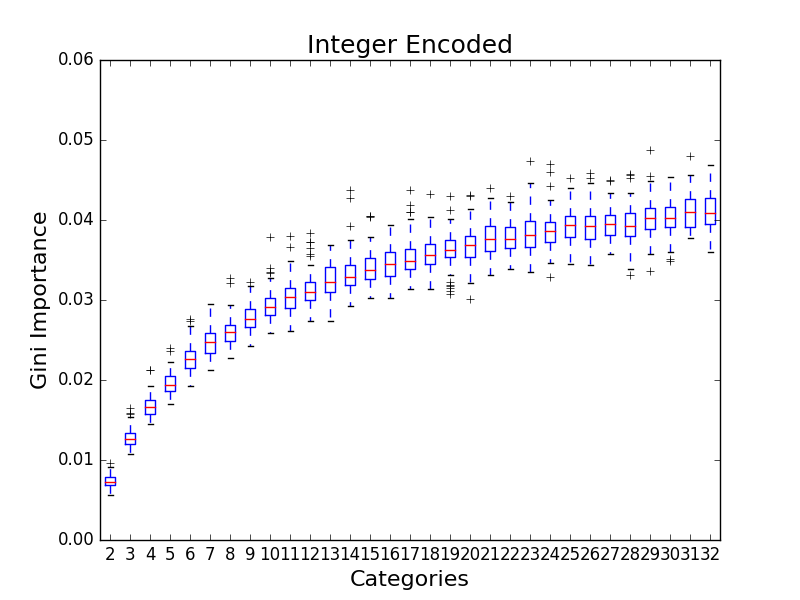
\includegraphics[width=\textwidth]{figures/random_forests/rf_bias_integer}
    \caption{Integer Encoded}
    \label{fig:integer}
  \end{subfigure}
  ~
  \begin{subfigure}[b]{0.45\textwidth}
    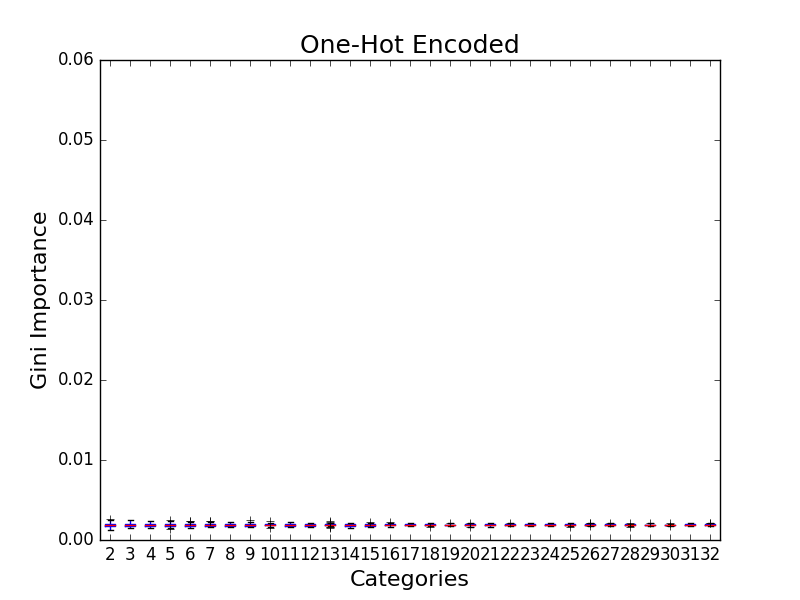
\includegraphics[width=\textwidth]{figures/random_forests/rf_bias_onehot}
    \caption{One-Hot Encoded}
    \label{fig:one-hot}
  \end{subfigure}

  Comparison of effect of encoding schemes for categorical variables on variable importance scores. The variables have randomly-chosen values with no correlation with output labels and 2-32 categories.
  \label{fig:encoding-schemes}
\end{figure}

\begin{figure}[H]
  \centering
  \caption{Effect of Missing Data on Variable Importance Scores}
  \begin{subfigure}[b]{0.45\textwidth}
    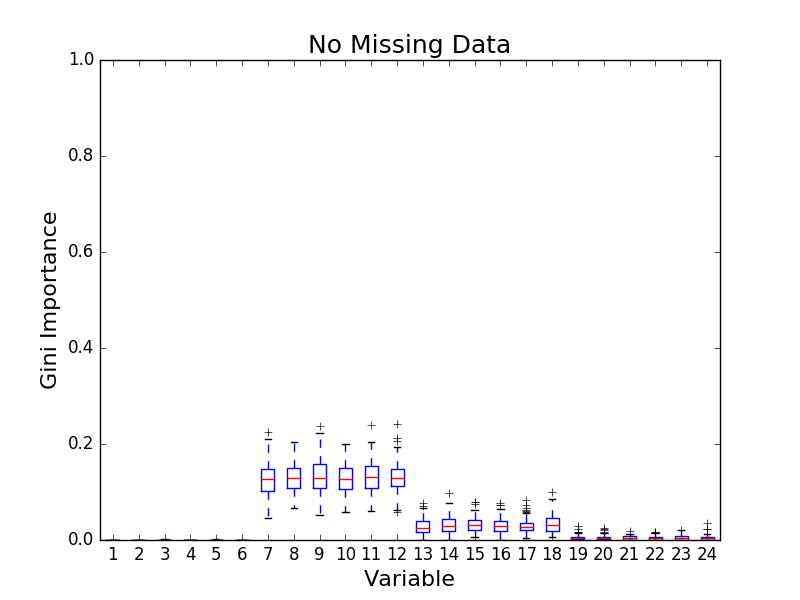
\includegraphics[width=\textwidth]{figures/random_forests/rf_missing_data_none}
    \caption{No Missing Data}
    \label{fig:missing-data-none}
  \end{subfigure}
  ~
  \begin{subfigure}[b]{0.45\textwidth}
    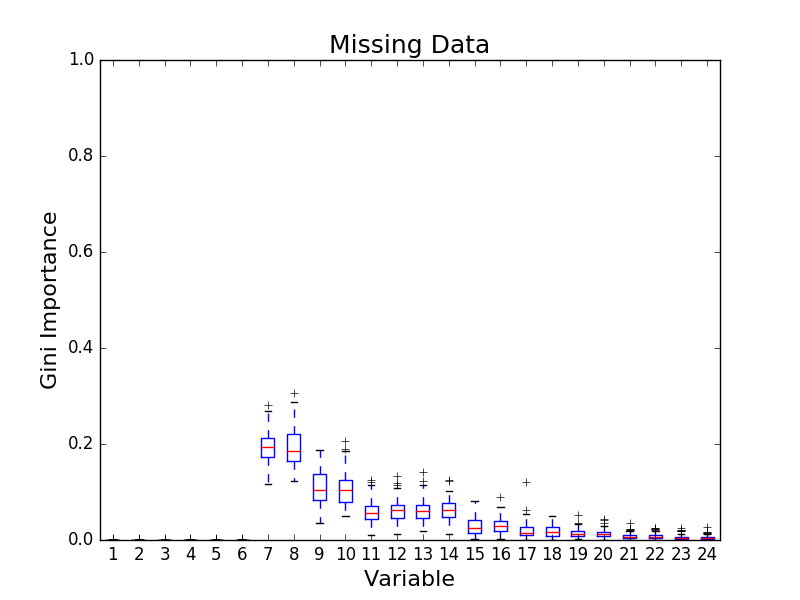
\includegraphics[width=\textwidth]{figures/random_forests/rf_missing_data}
    \caption{Missing Data}
    \label{fig:missing-data-missing}
  \end{subfigure}
  ~
  \begin{subfigure}[b]{0.45\textwidth}
    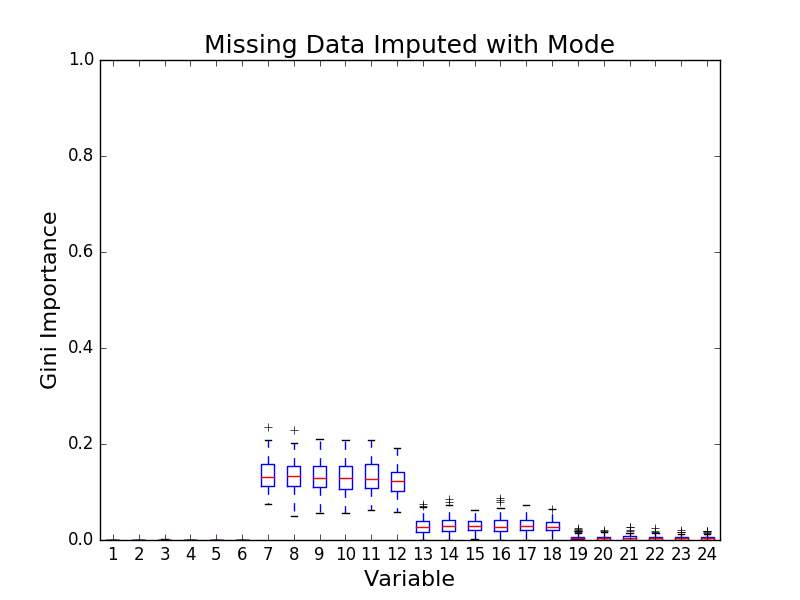
\includegraphics[width=\textwidth]{figures/random_forests/rf_missing_data_imputed_mode}
    \caption{Missing Data Imputed with Mode}
    \label{fig:missing-data-imputed}
  \end{subfigure}
  
  Effect of missing data on variable importance scores.
  \label{fig:missing-data}
\end{figure}

\begin{figure}[H]
  \centering
  \caption{Variable Importance Scores for Different Variable Counts}
  \begin{subfigure}[b]{0.45\textwidth}
    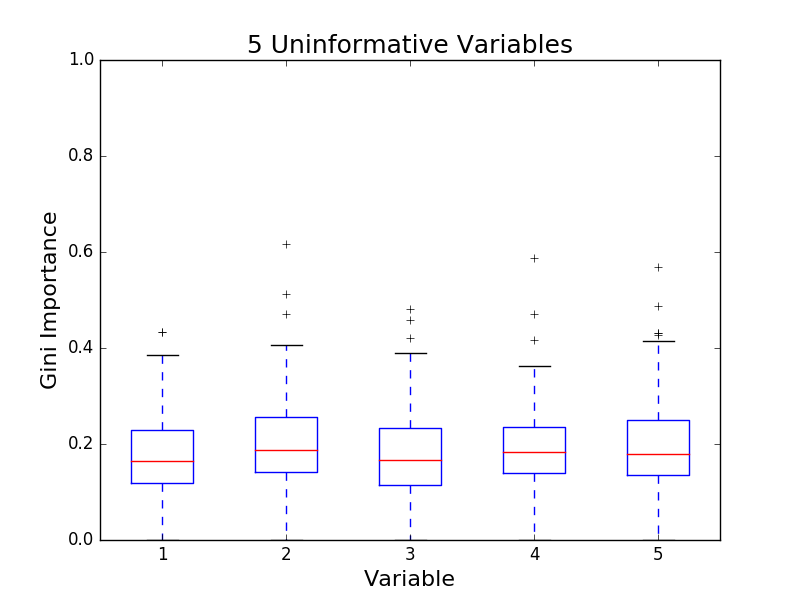
\includegraphics[width=\textwidth]{figures/random_forests/rf_variable_count_bias_5.png}
    \caption{5 Uninformative Variables}
    \label{fig:var-count-5}
  \end{subfigure}
  ~
  \begin{subfigure}[b]{0.45\textwidth}
    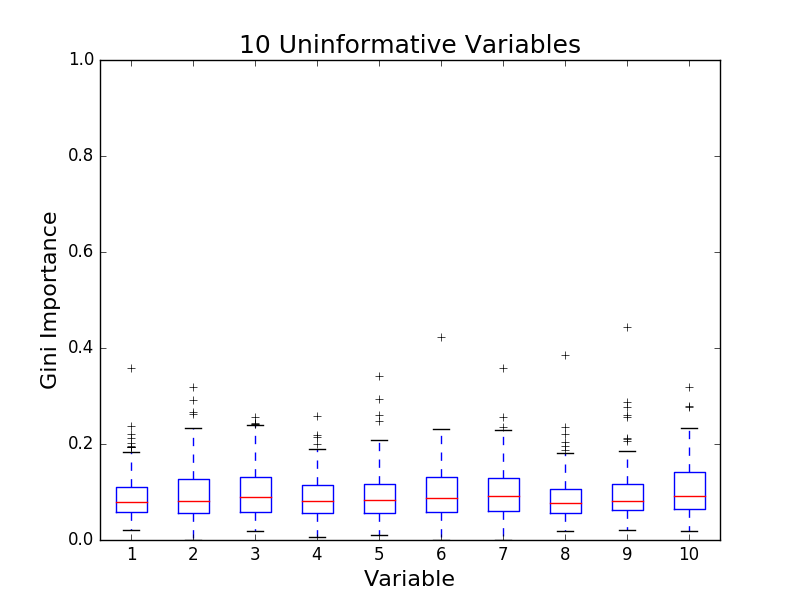
\includegraphics[width=\textwidth]{figures/random_forests/rf_variable_count_bias_10.png}
    \caption{10 Uninformative Variables}
    \label{fig:var-count-10}
  \end{subfigure}
  ~
  \begin{subfigure}[b]{0.45\textwidth}
    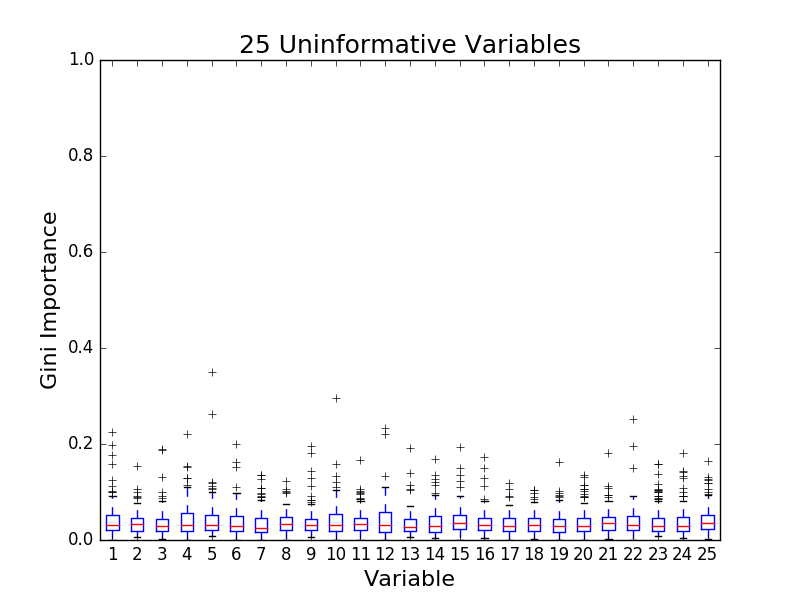
\includegraphics[width=\textwidth]{figures/random_forests/rf_variable_count_bias_25.png}
    \caption{25 Uninformative Variables}
    \label{fig:var-count-25}
  \end{subfigure}
  
  Distributions of variable importance scores with 5, 10, and 25 uninformative variables.
  \label{fig:var-count}
\end{figure}

\begin{figure}[H]
  \centering
  \caption{Different Numbers of Correlated Variables}
  \begin{subfigure}[b]{0.45\textwidth}
    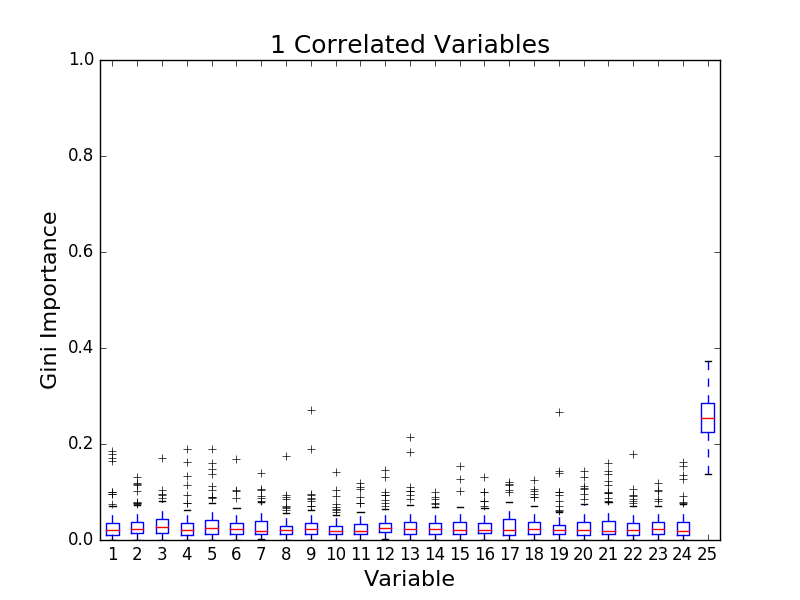
\includegraphics[width=\textwidth]{figures/random_forests/rf_correlated_1_0_1.png}
    \caption{1 Correlated Variable}
    \label{fig:corr-1-1}
  \end{subfigure}
  ~
  \begin{subfigure}[b]{0.45\textwidth}
    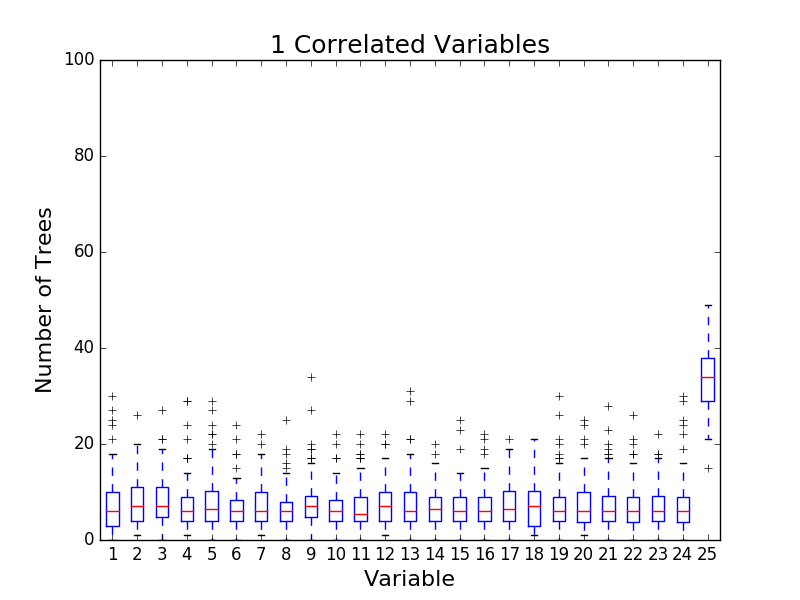
\includegraphics[width=\textwidth]{figures/random_forests/rf_correlated_1_0_1_feature_counts.png}
    \caption{1 Correlated Variable}
    \label{fig:corr-1-1-counts}
  \end{subfigure}
  ~
  \begin{subfigure}[b]{0.45\textwidth}
    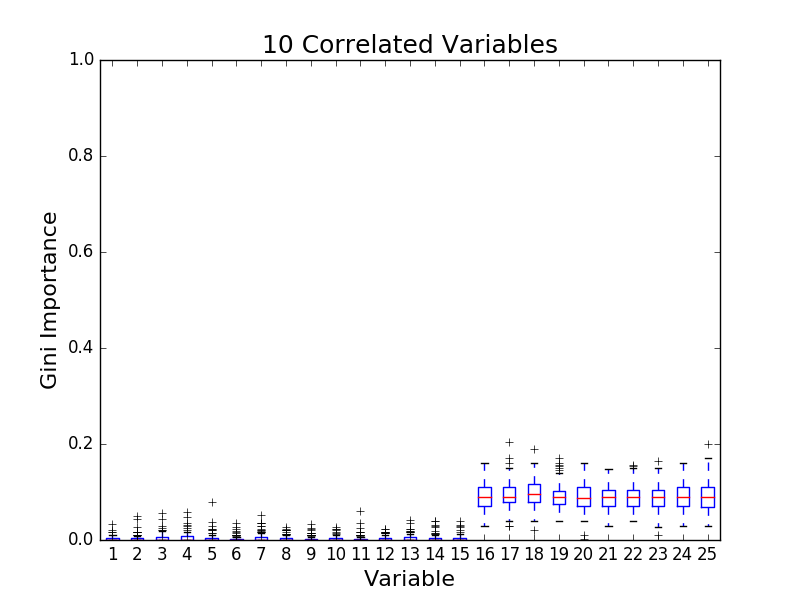
\includegraphics[width=\textwidth]{figures/random_forests/rf_correlated_1_0_10.png}
    \caption{10 Correlated Variables}
    \label{fig:corr-1-10}
  \end{subfigure}
  ~
  \begin{subfigure}[b]{0.45\textwidth}
    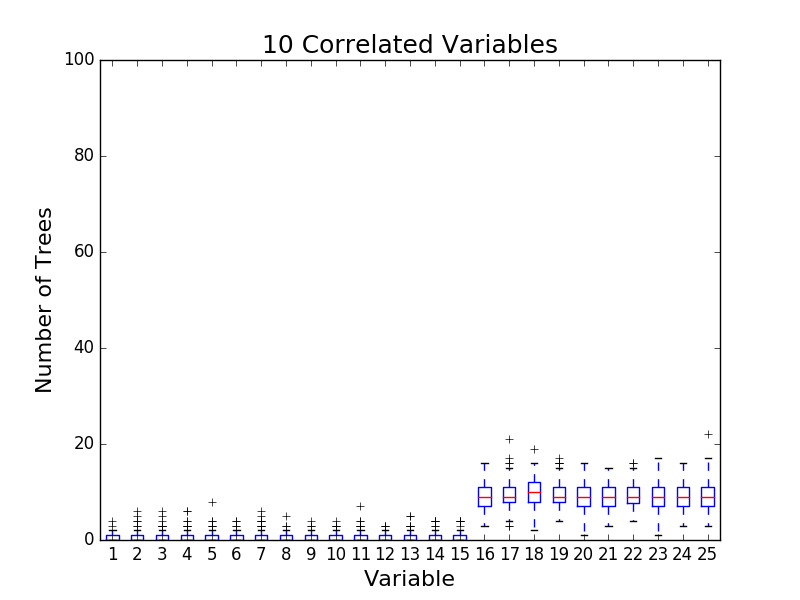
\includegraphics[width=\textwidth]{figures/random_forests/rf_correlated_1_0_10_feature_counts.png}
    \caption{10 Correlated Variables}
    \label{fig:corr-1-10-counts}
  \end{subfigure}
  ~
  \begin{subfigure}[b]{0.45\textwidth}
    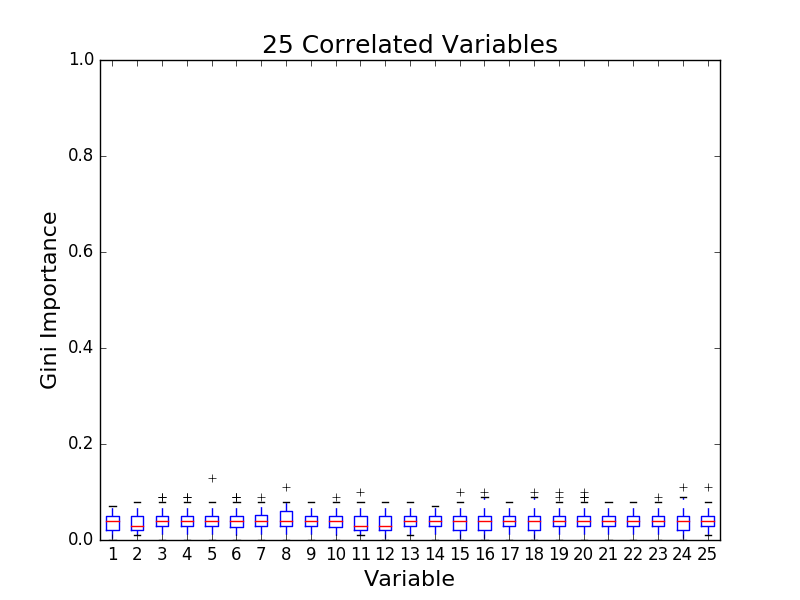
\includegraphics[width=\textwidth]{figures/random_forests/rf_correlated_1_0_25.png}
    \caption{25 Correlated Variables}
    \label{fig:corr-1-25}
  \end{subfigure}
  ~
  \begin{subfigure}[b]{0.45\textwidth}
    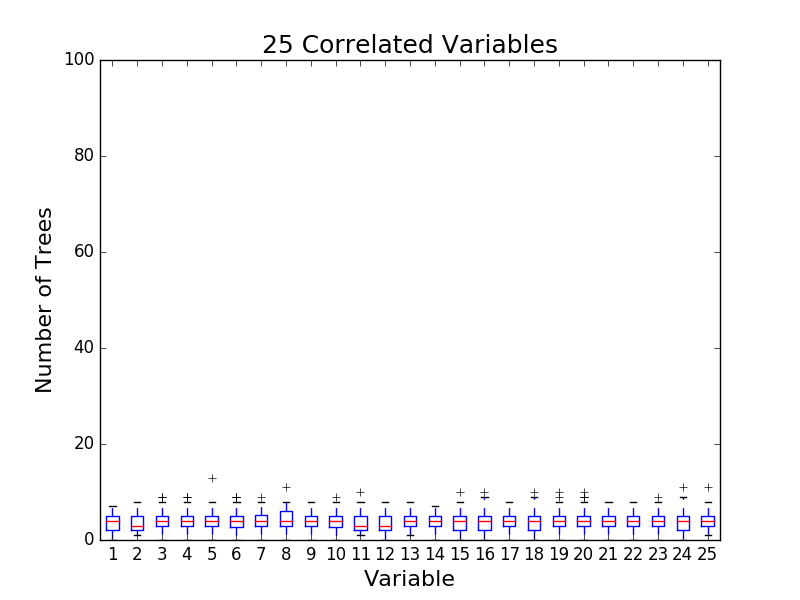
\includegraphics[width=\textwidth]{figures/random_forests/rf_correlated_1_0_25_feature_counts.png}
    \caption{25 Correlated Variables}
    \label{fig:corr-1-25-counts}
  \end{subfigure}
  
  Analysis of variables from generated data sets with 1, 10, and 25 out of 25 variables perfectly correlated with the output label. The left-hand side figures are distributions of variable importance scores. Right-hand side figures are number of trees using each variable.
  \label{fig:corr-1}
\end{figure}

\begin{figure}[H]
  \centering
  \caption{Mean Decrease in Impurity for Bagging and Constrained Bagging}
  \begin{subfigure}[b]{0.45\textwidth}
    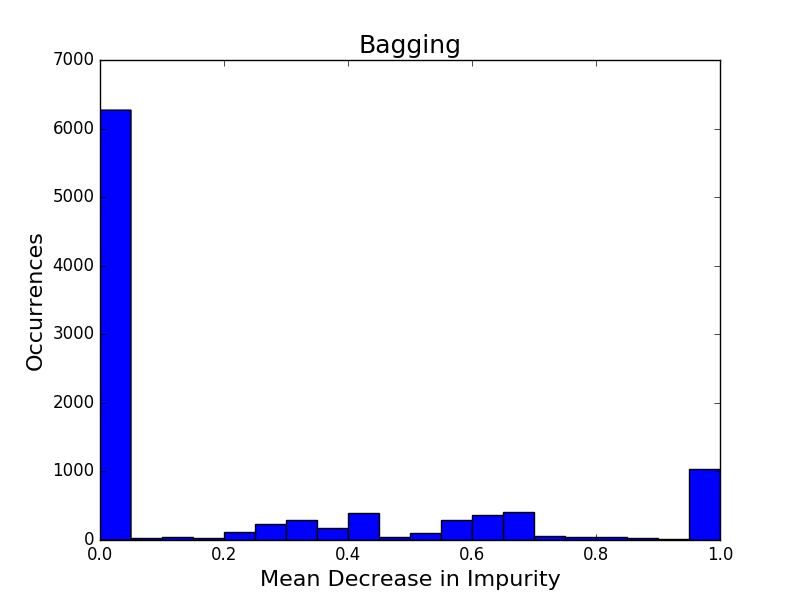
\includegraphics[width=\textwidth]{figures/random_forests/bagging_bias_bagging_hist.png}
    \caption{Bagging}
    \label{fig:bagging-bias-bagging}
  \end{subfigure}
  ~
  \begin{subfigure}[b]{0.45\textwidth}
    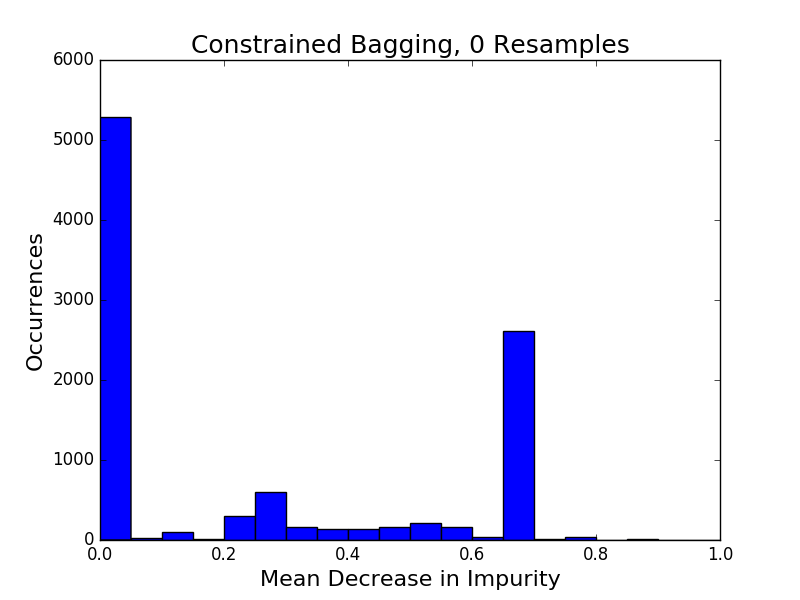
\includegraphics[width=\textwidth]{figures/random_forests/bagging_bias_no_bagging_hist.png}
    \caption{Constrained Bagging, 0 Resamples}
    \label{fig:bagging-bias-constrained-0}
  \end{subfigure}
  ~
  \begin{subfigure}[b]{0.45\textwidth}
    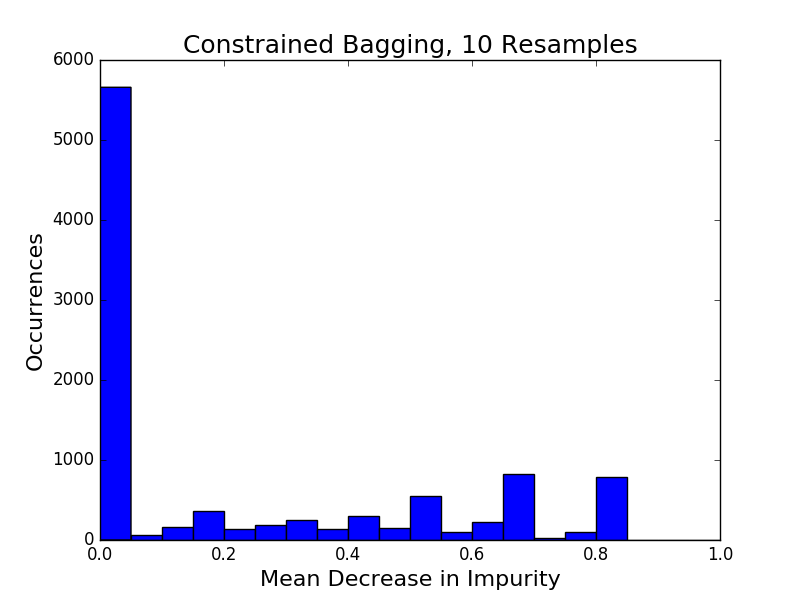
\includegraphics[width=\textwidth]{figures/random_forests/bagging_bias_constrained_bagging_hist_10.png}
    \caption{Constrained Bagging, 10 Resamples}
    \label{fig:bagging-bias-constrained-10}
  \end{subfigure}
  ~
  \begin{subfigure}[b]{0.45\textwidth}
    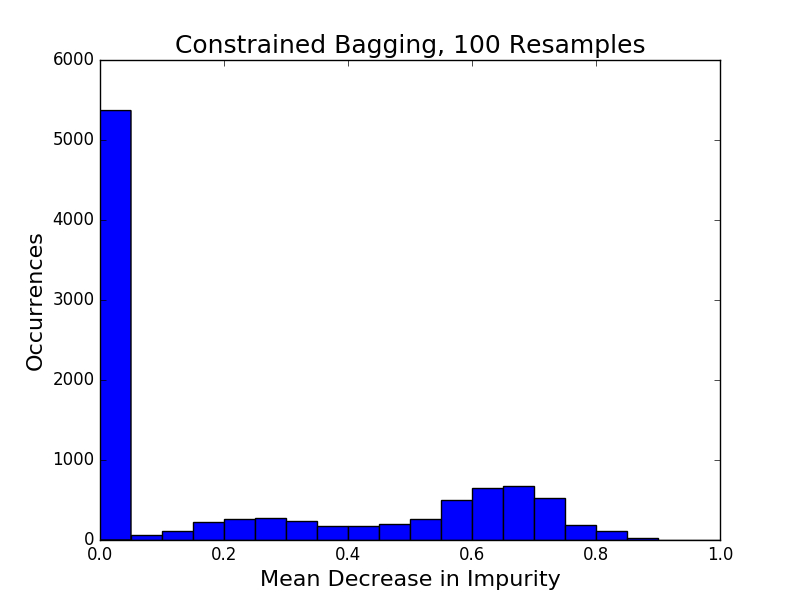
\includegraphics[width=\textwidth]{figures/random_forests/bagging_bias_constrained_bagging_hist_100.png}
    \caption{Constrained Bagging, 100 Resamples}
    \label{fig:bagging-bias-constrained-100}
  \end{subfigure}
  ~
  \begin{subfigure}[b]{0.45\textwidth}
    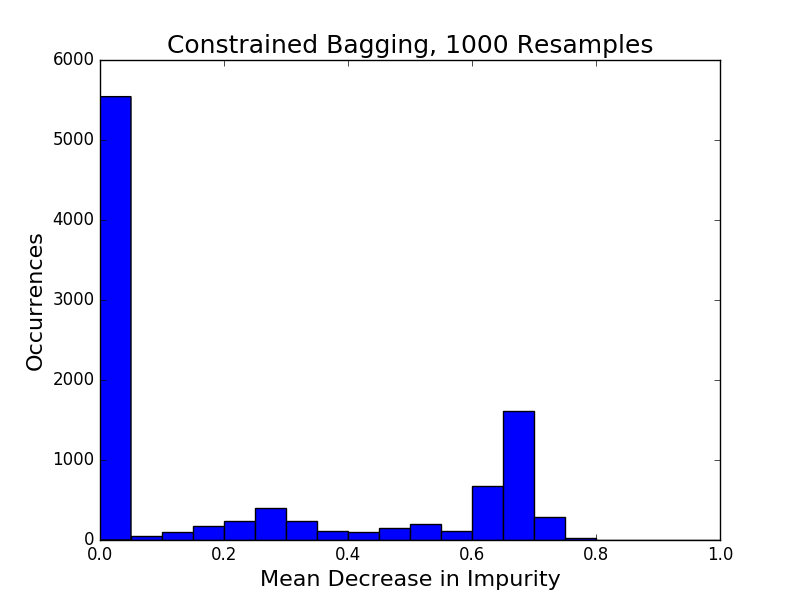
\includegraphics[width=\textwidth]{figures/random_forests/bagging_bias_constrained_bagging_hist_1000.png}
    \caption{Constrained Bagging, 1000 Resamples}
    \label{fig:bagging-bias-constrained-1000}
  \end{subfigure}

  Distributions of mean decreases in impurity when using bagging and constrained bagging with 0, 10, 100, and 1000 additional re-sampled instances.
  \label{fig:bagging-bias}
\end{figure}

\section{Tables}
\begin{table}[H]
  \begin{center}
    \caption{GENOTYPE EXAMPLES}
    \begin{tabular}{ c c c}
      \hline
      \textbf{Group} & \textbf{Before} & \textbf{After}\\ \hline
      1 & A/T & A/T \\
      1 & A/T & A/T \\
      1 & A/T & A/T \\
      1 & X/X & A/T \\
      2 & T/T & T/T \\
      2 & A/A & A/A \\
      3 & A/A & A/A \\
      3 & X/X & X/X \\
    \end{tabular}
  \end{center}
  
  Examples of two groups with known and unknown genotypes, before and after imputation with a threshold frequency of 100\%.
  \label{tab:unknown-genotypes-example}
\end{table}

\begin{table}[H]
  \begin{center}
    \caption{SNP EXAMPLES}
    \begin{tabular}{ c c c }
      \hline
      \textbf{Individual} & \textbf{(X, 1)} & \textbf{(X, 10)} \\ \hline
      1 & A/T & X/X \\
      2 & T/T & C/C \\
    \end{tabular}
  \end{center}

  Examples of SNP values for two individuals.  The SNPs are labeled by pairs of chromosome and position.
  \label{tab:encoding-example-snps}
\end{table}

\begin{table}[H]
  \begin{center}
    \caption{FEATURE MATRIX EXAMPLE}
    \begin{tabular}{ c c c c c c c }
      \hline
      \textbf{Individual} & \textbf{X, 1, A/A} & \textbf{X, 1, T/T} & \textbf{X, 1, A/T} & \textbf{X, 10, C/C} & \textbf{X, 10, G/G} &\textbf{X, 10, C/G} \\ \hline
      1 & 0 & 0 & 1 & 0 & 0 & 0 \\
      2 & 0 & 1 & 0 & 1 & 0 & 0 \\
    \end{tabular}
  \end{center}
  
  Feature matrix for the SNPs of two individuals.  The features are labeled by triplets of chromosome, position, and genotype.
  \label{tab:encoding-example-features}
\end{table}

